\part{Texto e Pós Texto}

\chapter[Revisão Teórica]{Revisão Teórica}
%\addcontentsline{toc}{chapter}{Revisão Teórica}

Nessa primeira parte do documento, objetiva-se explicitar com uma visão geral, os conceitos que existem por trás das aplicações de GNSS, bem como as aplicações que têm surgido a partir dessa tecnologia emergente.

Assim sendo, a primeira parte desse documento está dividida em 2 seções. Na primeira seção parte-se de um ponto de vista mais abrangente onde será exposto o estado da arte das tecnologias sistemas de navegação global por satélite, mostrando os rumos de desenvolvimento tanto de \textit{hardware} quanto de \textit{software} e as aplicações que têm surgido e fazem uso dessa tecnologia e suas técinicas.

Em seguida será abordado como de fato funciona o sistema de \textit{tracking} para o sistema GNSS considerado. Ali serão abordados o modelo de sinal considerado para implementação de desse sistema, bem como o ferramental matemático utilizado para a obtenção das informações de interesse.

\section{Estado da arte}

\cite{Antreich2022} associam o desenvolvimento e aprimoramento da tecnologia de sistemas GNSS ao desenvolvimento de semicondutores nessa nova era. Segundo esse autor, tal desenvolvimento possibilitou a miniaturização de compontnes, e aumentou o poder computacional de vários dispositivos eletrônicos. Exemplo claro disso é a possibilidade que um usuário de aplicativos de mensagem tem de compartilhar a sua localização atual, ou mesmo de compartilhar sua localização em tempo real com algum outro usuário.

Além de aplicações mais cotidianas e talvez reacreacionais, o avanço da tecnologia de GNSS possibilita o sensoriamento remoto de superfícies do planeta, como explica \cite{Zavorotny2014}. Utilizando do espalhamento do sinal transmitido de um satélite ao receptor e fazendo o processamento desses sinais que chegam com algumas diferenças de fase e frequência ao receptor, é possível obter informações tais como altitude e características o solo, como relevo, dureza, como mostra a \textbf{figura \ref{fig:dureza_do_solo_gráfico}}, ou propriedades dielétricas. Nessa figura é possível observar que a característica que se busca extrair vem de uma correlação que é feita entre os sinais enviado e refletido. No eixo vertical a potência dessa correlação é mensurada, de modo que altas correlações, região vermelha, indicam um solo mais macio; enquanto a baixa potência de correlação na região azul indicam um solo mais duro.

Ainda no que tange às aplicações, é possível citar os carros autônomos, que teêm ganhado grande evidência na atualidade. Sobre assunto, \cite{Cosart2020} ressaltam como atualmente a maioria dos carros possui sistemas de posicionamento já imbutidos em seus sistemas de interação com o usuário. Porém para que o nível de acurácia necessário à navegação de um carro completamente autônomo seja atingido, propõem um GNSS aumenado, que faz uso de outros recursos presentes nas cidades como radares e câmaras, o que proporcionaria esse aumento de precisão sem aumentar grandemente os custos com a tecnologia.

\begin{figure}[h] 
    \centering
    \caption{Gráfico para avaliar a dureza do  solo após processo de reflexão do sinal.}
    \label{fig:dureza_do_solo_gráfico}
    \includegraphics[width = 0.7\textwidth]{figuras/Gráfico para dureza do solo.png}
    
    Fonte \cite{Teunissen2017}
\end{figure}

Como visto anteriormente e ressaltado por \cite{Userreport2020} a migração do GNSS do meio exclusivo militar para o mercado em massa trouxe outras necessidades e desafios que motivam o avanço dessa tecnologia. Como começou a ser utilizada em ambientes diversos, cria-se a necessidade de sistemas que sejam adaptáveis tanto a ambientes internos quanto externos, urbanos e rurais. Além disso, com o crescente número de usuários, cria-se também a necessidade de se precaver contra roubo de acessos e interferência de sinal. E como esses novos acessos não são contíuos, ao atingirem um dado objetivo os sistemas são desativados e só serão ativados em uma outra ocasião, é necessário também que o tempo para que o receptor fixe a posição dos satélites, \textit{time to fix (TTF)}, seja o menor possível. 

Assim, para que esses objetivos sejam alcançados, é necessária a evolução conjunta das diversas partes que compõem os receptores desses sinais. Na \textbf{figura \ref{fig:GNSS_components}} é possível ver os componentes da arquiterura desses receptores, desde a antena e recepção em rádio frequências ao processamento dos sinais. Para que haja o aumento de precisão dos sinais e crie-se a robustez necessária, não basta que um desses componentes seja aprimorado sem que o restante o acompanhe. Assim, a parte final dessa seção se dedica a mostrar os avanços e desafios encontrados em cada parte dos componentes dessa teconologia. 

Seguindo a estrutura de recepção apresentada na \textbf{figura \ref{fig:GNSS_components}}, nota-se que todo o processo começa na antena de recepção. Diversos são os desafios que estão presentes nesse estágio da recepção do sinal. \cite{Antennas2012} destaca dois principais desafios no projeto dessas antenas: largura de banda e restrição de tamanho imposta pela plataforma.

\begin{figure}[h]
    \centering
     \caption{Arquitetura clássica, a nível de componentes, de um receptor GNSS}
    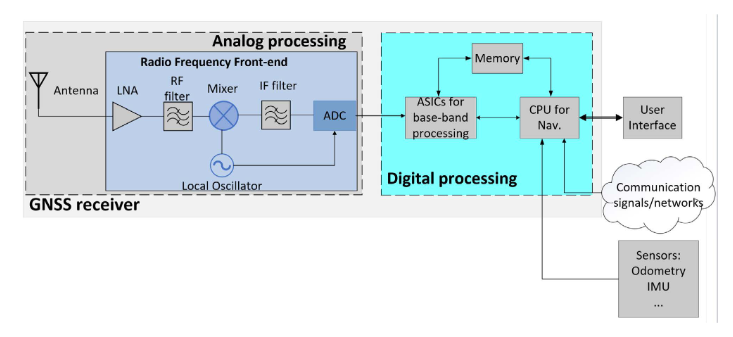
\includegraphics[width = 0.7\textwidth]{figuras/GNSS_componentes.png}
    
     Fonte: \cite{Antreich2022}
    \label{fig:GNSS_components}
\end{figure}

\cite{Teunissen2017} explicam que o sistema americano de GNSS, o GPS, está centrado em 3 frequências: L1, L2 e L5, a saber, 1.575GHz, 1.227GHz e 1.176GHz, respectivamente. Entrtanto, apesar de estar centrado nessas frequências, os receptres precisam ter uma largura de banda de $\pm 10.23 MHz$. Essa largura interfere na capacidade de transmitir e receber informações do satélite com que se comunica. Uma banda mais estreita comprometeria o sistema a taxas inferiores na sua comunicação, tornando-a menos eficiente, por isso ter uma largura de banda adequada é crucial.

Entretanto, \cite{Antennas2012} explica que atingir a largura de banda necessária e respeitar os limites impostos pela plataforma são requisitos conflitantes, uma vez que estão limitados fisicamente. Toda a geometria e tamanho da antena interferem na sua largura de banda, e quando se é necessário fazer a miniaturização da antena, acaba-se por causar ressonâncias em frequências mais baixas, diminuindo a largura de banda da antena, como explica \cite{Antreich2022}.

Assim, é necessário que haja um compromisso entre as caracaterísticas desejadas para a antena do sistema. E atualmente as antenas de microfita têm feito um bom balanço dessas caracterísicas, uma vez que são discretas e possuem uma considerável ganho de performance, entretanto para que possuam uma largura de banda maior, é necessário que se faça uma sobreposição de camadas, como explica \cite{Teunissen2017}, o que pode não atender às restrições da plataforma utilizada.

Em seguida, ainda de seguindo o esquema da \textbf{figura \ref{fig:GNSS_components}}, após a antena existe a unidade de processamento analógico. É possível observar que essa parte do receptor é composta por um LNA, \textit{Low Noise Amplifier}, Amplificador de baixo ruído, que amplifica o sinal do satélite, seguido de dois filtros, que ajudam a remover os ruídos de frequências indesejadas. Nessa toada, cabe ressaltar que os componentes em si podem introduzir ruídos no sistema de diversas formas, como ruído térmico, o que dificulta a percerpção e tratamento do sinal que é recebido. A função do LNA, portanto é de ampliar esse sinal que chega, mas procurando introduzir a menor quantidade de ruído possível, porém há de se saber que exisitirá uma certa quantidade de ruído injetada. E justamente para controlá-lo existem os filtros passa-faixa que seguem o processo de amplificação na cadeia de recepção. Sabendo-se a faixa de frequências do sinal de interesse, esses filtros atenuarão frequências vizinhas, de modo que o sinal anteriormente amplificado fique ainda mais limpo. Por fim, estão o oscilador local e o conversor analógico para digital. 
 
Ademais, cabe ressaltar que os osciladores são componentes em Hardware, ou seja, enfrentam defeitos e imperfeições inerentes a componentes que são fabricados e montados. O oscilador funciona com um cristal interno e apartir das oscilações desse cristal, são produzidas as oscilações utilziadas no processamento em software. Essas oscilações, como explicita \cite{Antreich2022}, estão diretamente relacionadas com a temperatura e quanto mais estável a temperatura, mais estáveis as oscilações de clock produzidas pelo oscilador. Fica bem claro que esse é o principal desafio no que tange aos osciladores em hardware, uma vez que estabelecer controles mais sutis de temperatura tonam mais caro o processo de produção de receptores para o mercado em massa.

No último estágio do processamento analógico está o conversor analógico-digital. A fim de fazer essa conversão, é necessário que seja feita uma amostragem do sinal analógico da entrada. Essa amostragem em si requer certo poder computacional, mas dependendo do tamnho das amostras necessárias para se conseguir amostrar o sinal com uma grande quantidade de ruído, mais poder computacional será requerido para processar o tamnho da amostra. Nesse caso há de se fazer um compromisso entre o consumo de energia e memória ea necessidade de precisão na aplicação em que o sinal processado será utilizado.

Finalmente, ao final da cadeia de recepção apresentada na \textbf{figura \ref{fig:GNSS_components}}, observa-se a cadeia de processamento digital. Nessa cadeia exitem dois componentes principais: o módulo de aquisição e o de \textit{tracking}. O objetivo do módulo de aquisição é fazer uma primeira estimativa dos parâmetros de atraso e doppler do sinal. Essa é uma estimação grosseira desses parâmetros. Entretanto, por lidar com velocidades na ordem de $10^8$, pois são ondas eletromagnéticas, erros podem representar metros de erros, assim, é necessário que uma estimativa mais refinada seja feita. É para essa função que existe o sistema de \textit{tracking}.

Cabe ressaltar que o estudo do bloco de \textit{tracking} é o principal assunto deste documento. \cite{Antreich2022} ressalta que a perspectiva de evolução para esses módulos está na miniaturização e também no uso de memória por parte dos chips de prochessamento. Uma vez que os usos de mercado do GNSS estão necessitando de mais precisão, é necessário mais disponibilidade de memória para acumular correlações mais precisas.

Por fim, é possível notar que a tecnologia de \textit{Global Navegation Satellite Systems}, por mais consagrada que seja, ainda possui espaço para otimizações e melhorias, que surgem da demanda que o mercado em massa, isto é o uso comercial e cotidiano, tem requerido desses sistemas. Desde a cadeia analógica à digital, é possível encontrar espaço e oportunidadespara aperfeiçoamento dessas tecnologias que vêm ganhando mais espaço e aplicações no cotidiano.

Agora, esse trabalho se dedica a demonstrar o funcionamento das partes necessárias ao entendimento do sistema de \textit{tracking} e sua operação.